\documentclass[12pt]{article}

\usepackage[english]{babel}
\usepackage[utf8x]{inputenc}
\usepackage{pdfpages}
\usepackage{lastpage} % Required to determine the last page for the footer
\usepackage{extramarks} % Required for headers and footers
\usepackage{graphicx} % Required to insert images
\usepackage{listings} % Required for insertion of code
\usepackage{courier} % Required for the courier font
\usepackage{color}
\usepackage{grffile}
\usepackage{float}

\usepackage[a4paper, total={6in, 8in}]{geometry}

% Margins
\topmargin=-0.45in
\evensidemargin=0in
\oddsidemargin=0in
\textwidth=6.5in
\textheight=9.0in
\headsep=0.25in
\fboxsep=0mm%padding thickness
\fboxrule=2pt%border thickness

\linespread{1.1} % Line spacing

\newcommand{\Title}{Software Documentation Document} % Assignment title
\newcommand{\Class}{Cos\ 301} % Course/class
\newcommand{\pd}{Post-Doctoral}
\newcommand{\ssr}{Soft\color{green}{Serve }\color{black}}
\newcommand{\version}{0.9}
\newcommand{\iteration}{1}
\newcommand{\client}{Ms. Cathy Sandis (UP Research Office)}
\newcommand{\project}{Post-Doctoral Application Management System}

\begin{document}


\vspace{4em}

\begin{center}%

\begin{figure}[ht!]
\centering

\includegraphics{../Images_Docs/logo.png}
\end{figure}
\LARGE \bf \project \\[1em]
\LARGE \bf \Title \\[0.25em]
\large \bf \today\\
\bf Version \version\\
\bf Iteration \iteration\\[0.5em]
\Large \bf Prepared for \client\\
\Large \bf by
\Large {\bf \ssr Group }\\[0.5em]
\LARGE {\bf Group members}\\[0.25em]
\large
Kgothatso Phatedi Alfred Ngako (12236731) \\[0.5em]
Tokologo “Carlo” Machaba (12078027) \\[0.5em]
Mathys Ellis (12019837) \\[8em]

\end{center}%

%\newpage
%{\LARGE \bf Change log}\\[2em]

\begin{center}
\begin{tabular}{|l|p{1.4cm}|p{8cm}|p{2.8cm}|}
\hline
\multicolumn{4}{|c|}{\bf Change log} \\
\hline
 Date & Version & Description &  Person \\
\hline
18/05/2014 & v 0.0 & Document created. & Alfred Ngako \\
\hline
19/05/2014 & v 0.0 & Added more detail to information in subsections. & Alfred Ngako \\
\hline
20/05/2014 & v 0.0 & Added references and citations. & Alfred Ngako \\
\hline
%\end{tabbing}
\end{tabular}
\end{center}
\newpage
\tableofcontents

\listoffigures
\newpage
%%%%%%%%%%%%%%%%%%%%%%%%%%%%%%%%%%%%%%%%%%%%%%%%%%%%%%%%%%%%%%%%%%%%%%%%%%%%%%%%%%%%%%%%%%%%%%%%%%%%%%%%%%%%%

\section{Document description:}%Not entirely sure what I should add here

\subsection{Document purpose}
\vspace{0.2in}
This document provides the documenting for the software architecture infrastructure which the application functionality is deployed and executed.

\vspace{0.2in}

\subsection{Documentation methodology}
\vspace{0.2in}
\begin{flushleft}
The documentation and software development methodology used by the project adhere to the guidelines set out by the agile method. Thus this document has undergone and will undergo various iterations that may extend or reduce the contents of the document.\\

The document was compiled using a software architecture specification document template provided by Dr Fritz Solms as an alternative to the Kruchten 4 + 1 approach to documenting software.

This document was created using the requirement elicitation techniques and requirement definitions as specified by Klaus Pohl’s book Requirements Engineering: Fundamentals, Principles, and Techniques [Dr.Phol, K., 2010].
The requirements, vision and scope were elicited from the following sources:
\begin{itemize}
	\item Numerous interviews with the client.
	\item On-line research into UP Post doctoral applications.
	\item Correspondence with the UP IT department.
	\item Collecting and analysing various documents such as:
		\begin{itemize}
			\item The initial project request document
			\item Application forms
			\item Renewal forms
			\item CV templates
			\item Approval and recommendation forms
		\end{itemize}
\end{itemize}
\end{flushleft}	

\vspace{0.5in}

\subsection{Document conventions:}
\vspace{0.1in}
\begin{itemize}
\item Documentation formulation tool: LaTeX
\end{itemize}

\vspace{0.2in}

\subsection{References:}
\vspace{0.1in}
\begin{itemize}
\item Dr.Phol, K., 2010, \textit{Requirements Engineering: Fundamentals, Principles, and Techniques}, Springer, Heidelberg.
\item Abraham Kang. Aug 9, 2002, \textit{Enterprise application integration using J2EE}, Available from: http://www.javaworld.com/article/2074488/enterprise-java/enterprise-application-integration-using-j2ee.html , [17 May 2014]
\item Jendrock E, Cervera-Navarro R, Evans I, Haase K, Markito W, \textit{The Java EE 7 Tutorial}, Available from: http://docs.oracle.com/javaee/7/tutorial/doc/home.htm , [20 May 2014]
\end{itemize}	

\vspace{0.5in}

\newpage

%%%%%%%%%%%%%%%%%%%%%%%%%%%%%%%%%%%%%%%%%%%%%%%%%%%%%%%%%%%%%%%%%%%%%%%%%%%%%%%%%%%%%%%%%%%%%%%%%%%%%%%%%%%%%
\section{Architecture Requirements} 
This section discusses the software architectural requirements from the software requirements such as:
\begin{itemize}
\item Architectural Scope,
\item Quality Requirements,
\item Integration and Access Channel Requirements, and
\item Architectural Constraints.
\end{itemize}
All the above mentioned topics are put in place to address the non-functional requirements that were illicited from \client .

%%%%%%%%%%%%%%%%%%%%%%%%%%%%%%%%%%%%%%%%%%%%%%%%%%%%%%%%%%%%%%%%%%%%%%%%%%%%%%%%%%%%%%%%%%%%%%%%%%%%%%%%%%%%%
\subsection{Architectural Scope}
The scope that the architecture needs to cover include:
\begin{itemize}
\item A persistence infrastructure (Database) to facilitate domain objects (e.g CVs, DRIS information, and Applications). This will also allow the implementation of the Audit trail required by the client and the centralised point for all the required documentation shared among stakeholders.
\item A session oriented infrastructure to assist in realizing the security requirements of authenticating participants and their actions.
\item A web access channel which will provide the client, and other stakeholders, with an interface to the underlying system.
\item An infrastructure for the generation of reports.
\item A mailing competent infrastructure.
%\item Data export... (completed applications to be sent to) % What to say here
%\item Pipe line infrastructure?????? % What about this as well?
\end{itemize}

%%%%%%%%%%%%%%%%%%%%%%%%%%%%%%%%%%%%%%%%%%%%%%%%%%%%%%%%%%%%%%%%%%%%%%%%%%%%%%%%%%%%%%%%%%%%%%%%%%%%%%%%%%%%%
\subsection{Quality Requirements} 
\vspace{0.2in}
The following are the requirements around the quality attributes of the systems and the services it provides:
These are the quality requirements as specified by the client and are also in the order of precedence. Where the first takes the highest precedence.

\subsubsection{Usability requirements}

\begin{flushleft}

This is first and foremost quality requirement stipulated by the client. The primary language of the system will be South African English. Any other language support is not considered part of the requirements but the system will be designed to allow for such development in the future.\\

\vspace{0.1in}

The system's UI will only consider 2 types of user categories with regard to usability:

\begin{itemize}

\item\textbf{Trained user:}

This type of user will have to have training in understanding how the system functions and how to use it. Their computer skills will be assumed to be in the range of basic to intermediate. Thus the user interface can allow for certain complexities but these complexities must be kept at a minimal. These user will be regarded as system administrators or specialised users of the system. The stakeholders who fall under this category is the DRIS staff members overseeing the application process and any technical or maintenance support users.

\item\textbf{Normal user:}

This type of user will have no training with regard to the system. Their computer skills will be assumed to be none or minimal. Therefore the UI that they will have access to will be simplistic and will be as user friendly as possible. The stakeholders that fall under this category will be Prospective fellows, Research fellows, Referees, Grant holders, HODs, Dean's office members and Post-doctoral committee members.

\end{itemize}

In order to quantify the above the SoftServe group will need to provide the system with a uniform user experience that is as simplistic and as visually oriented as possible without negating the below requirements severely. In addition to this any form of help text or instruction should be written in as natural, uncomplicated and unambiguous manner as possible. 

\end{flushleft}

\subsubsection{Security requirements}

\begin{flushleft}

The system will need to be fully secured since it deals with confidential information such as person information, application statuses, financial data and meeting information. Also since the systems main goal is to provide stable and audible application and renewal process flow the system may not be vulnerable to data tampering or any tampering whatsoever. It should be noted that this requirement conflicts with the Usability requirement above as it is known that the more secure a system becomes the less user friendly it becomes. Therefore the SoftServe group will try to balance the two requirements in such a way that neither of the two is negated.\\
\vspace{0.1in}

The system will have to provide different security roles to the registered users on the system. Any number of roles should be assignable to any user by a system administrator to allow for flexibility.\\
There will also need to be predefined roles so to allow a stakeholder from list of stakeholders in the vision and scope document, to only have the ability and access to perform the actions as defined by the vision and scope document.\\
The system administrator should be able to access all the sections in the system and should be able to modify them except where only the system itself has that right.\\
Another security requirement is that the audit trail must not be allowed to be modified by any human user and only allow the system to be able to insert data into the audit log. Further the audit table should only allow be query-able by a user with the correct security role.\\
To further quantify this requirement the system must provide some means of a centralised user authentication that acts as a gateway for all users of the system. Also every time some action is made by the user the user needs to be re-authenticated to insure that the user does have the correct privileges and if any user account changes where made it takes immediate affect. \\
Any form of account retrieval token or on-demand user account creation tokens must expire within a specified time period. For account retrieval token this should be 1 hour. For on-demand user account creation this should be about 2 days.

\end{flushleft}

\vspace{0.1in}

\subsubsection{Auditability:}

\begin{flushleft}

This is seen as the third most important requirement according to the client. The system needs to provide some form of an audit trail of all critical actions that occur in the system. Critical actions are considered: user account management operations, login action, logout action as well as any operation by a user that leads to a change in the data stored by the system. The Audit trail will be in the form of a read-only table stored in the database as stipulated in the security requirements above.\\

To quantify this requirement, the system will need to have an active audit log that can capture all the actions, that meet the list of critical actions, of each user that uses the system. With regards to usability, the feature needs to run in the background and not be noticeable by any user while they are using the system except if it is deliberately queried.

\vspace{0.1in}

\end{flushleft}

\subsubsection{Scalability requirements}

\begin{flushleft}

As research is still viewed as small field that is slowly growing by the client this is only the fourth most important requirement for the system. The current aim is to create a scalable system that can support 50 to 500 applicants per year with possible growth to a 1000 or more. This is in line with the figures given by the client and the growth, over the next ten to twenty years, in the research sector of the University of Pretoria.\\
\vspace{0.05in}

The system needs to be scalable in regard to the following factors:
\begin{itemize}

\item\textbf{Performance:} This aspect of the system regards the speed and responsiveness of the system.
The system needs to be handle large report queries in less than 10 seconds. It should be able to handle any application approval service processing in less than 3 seconds. It should be able to send emails instantly from the system side. Note this may be difficult to measure due internet bandwidth and receiving mail server constraints. Login, logout and user authentication should be handled in less then a second by the system this does not  considering the transfer of data to and from the server which is depended on the network connection speed.\\

\item\textbf{Storage:} This aspect of the system regards the growth and shrinking of the data that is stored by the system.
The system will need to be able to handle a database that is in the range of 1 GB to 15 GB that has the potential to grow even larger. The reason for this stems from the fact that the system will need to store a large amount of active data over a period of about 3 to 8 years before it can be archived.
\\Another requirement of the system is that it will need to support archival functionality and archived data that will eventual store all the old data from the active database for as long as time period as possible. Since the archival database should only grow it will need to be about 15 times larger than the active database. Due these reasons the calculation of how much space should be required will only be possible once the system is implemented and practically tested.\\The suggested linear formula to the above analysis is as follows: 
\begin{equation}
A \times ( (Xna \times Nna) + (Xra \times Nra) ) = B
\end{equation}

A = Number of years for which archival or active support is intended\\
B = Number of bytes needed on average for A years\\
Xna = Average number of bytes per new application\\
Xra = Average number of bytes per renewal application\\
Nna = Number of new applications a year\\
Nra = Number of renewal applications a year\\

\item\textbf{Concurrency:} This regarded as the amount of active users on the system at the same time.
The system will need to support at least 100+/- concurrent users efficient and effectively since the system requires multiple stakeholders to part take in the application process while there can be multiple applications occurring at the same time.\\

\end{itemize}
\end{flushleft}
\vspace{0.1in}

\subsubsection{Availability:}

\begin{flushleft}

The system's availability on designated networks will depend on the availability of the University of Pretoria's servers or whatever hosting service that will used to host the system. It should be noted that the former will only be possible if the project is considered acceptable by the UP's IT department.\\
In order to quantify this it should be seen as follows: If the hosting service's servers hosting the system are active and provide access over a designated network then the system must be available over that designated network. Where the designated networks are defined as the internet and/or the local network where in the server of the hosting service is located.

\end{flushleft}

\vspace{0.1in}

\subsubsection{Testability:}

\begin{flushleft}

The system must be testable. This will be done using unit testing and following the test plan that will be laid out in the testing document of this project.\\

\vspace{0.1in}

Unit testing will test each unit in regard to:
\begin{itemize}

\item\textbf{Preconditions}
\item\textbf{Post conditions}

\end{itemize}

The project will also have two phases of testing:

\begin{itemize}

\item\textbf{Offline:} This is the initial phase of testing and debugging which will be done with pseudo data.
\item\textbf{Online:} This is the final phase of testing and debugging which will be done with active real time data.

\end{itemize}

\end{flushleft}

\vspace{0.1in}





\vspace{0.1in}	



\vspace{0.2in}

\subsubsection{Robustness:}

\begin{flushleft}

This requirement was identified by the SoftServe group as being very important since the system will be receiving and handling large amounts of sensitive data. Thus the integrity of the data must be insured. To do this the system needs to be robust in in terms of its data storage routines, security routines and data validation, system integrity. 

These four aspects of robustness are quantified as follow:
\begin{itemize}
\item \textbf{Data storage}: When data is stored the data needs to be validated against a set of storage rules and constraints. Many DBMS packages allow this type of validation through data typing and allowing the database administrator to a specify constraints.
\item \textbf{Security}: As mentioned above in the security requirements the re-authentication of users is required and any form of account retrieval token or on-demand user account creation tokens must expire within a specified time period and that as only one token may be active at a time.
\item \textbf{Data validation}: All data that is manually imputed by a user, such as text, numbers, emails, passwords, etc. Must be checked to see if they meet constraints imposed on them through the use of data type checking and regular expression analysis. Any section in the system that requires certain data to completed before performing a action must be checked for completeness before allowing the user to perform the action. Where completeness means the data is not empty and validate according to constraints imposed on it.
\item \textbf{System Integrity}: If there are any defects with any other components with in the system and a task cannot be completed the user will also be notified immediately with the appropriate message sent to them.
\end{itemize}


\end{flushleft}

\vspace{0.1in}

\vspace{0.2in}

\subsubsection{Flexibility:}

\begin{flushleft}

The system is designed in such a way that adding new features can be done without extensive code restructuring. The process of adding new features will require the programmer to create a new module for the new functionality.

\end{flushleft}

\vspace{0.1in}

\vspace{0.2in}

\subsubsection{Reusability:}

\begin{flushleft}

The System's components will be used again where applicable. The Login credentials is an example of areas where the system will be reused.

\end{flushleft}

\vspace{0.1in}

\vspace{0.2in}

\subsubsection{Maintability:}

\begin{flushleft}
The system administrator will have the responsibility of adding updates that a programmer may wish to add to the system. 

\end{flushleft}

\vspace{0.1in}


%%%%%%%%%%%%%%%%%%%%%%%%%%%%%%%%%%%%%%%%%%%%%%%%%%%%%%%%%%%%%%%%%%%%%%%%%%%%%%%%%%%%%%%%%%%%%%%%%%%%%%%%%%%%%
\subsection{Integration and Access Channel Requirements}
This section discusses 
\begin{enumerate}
\item the requirements for the different channels through which the system can be accessed by humans and other system, and
\item the integration channels which must be supported by this system.
\end{enumerate}

\subsubsection{Access Channels}
The system must be reachable securely through a web browser. 

\subsubsection{Integration Channels}
Upon completion the system must be integratable with the University of Pretorias PeopleSoft system.

%%%%%%%%%%%%%%%%%%%%%%%%%%%%%%%%%%%%%%%%%%%%%%%%%%%%%%%%%%%%%%%%%%%%%%%%%%%%%%%%%%%%%%%%%%%%%%%%%%%%%%%%%%%%%
\subsection{Architectural Constraints}
\client did not specify any Architectural constraints other then the fact that the system must be integratable with the University of Pretoria, packaged software solution, PeopleSoft System. 

% 
%%%%%%%%%%%%%%%%%%%%%%%%%%%%%%%%%%%%%%%%%%%%%%%%%%%%%%%%%%%%%%%%%%%%%%%%%%%%%%%%%%%%%%%%%%%%%%%%%%%%%%%%%%%%%
\section{Architectural Patterns and Styles} % skipped till further notice.

% Mention of how Java EE actually doesn't require use of GoF design patterns >> http://www.theserverside.com/tip/With-Java-EE-7-your-Design-Patterns-are-dead-And-your-EAR-is-ugly-too <<

The system will maintain a MVC architectural pattern specific to how Java EE is structured. Which is a layered structure that automatically decouples the client from the server.\\
\\
The Java EE structure is designed to satisfy the need for distributed, transactional, and portable applications that leverage the speed, security, and reliability of server-side technology. Which is reason to why it suits its use in the development of the system. The following diagram provides the abstracted architectural structure which will be followed:
\begin{figure}
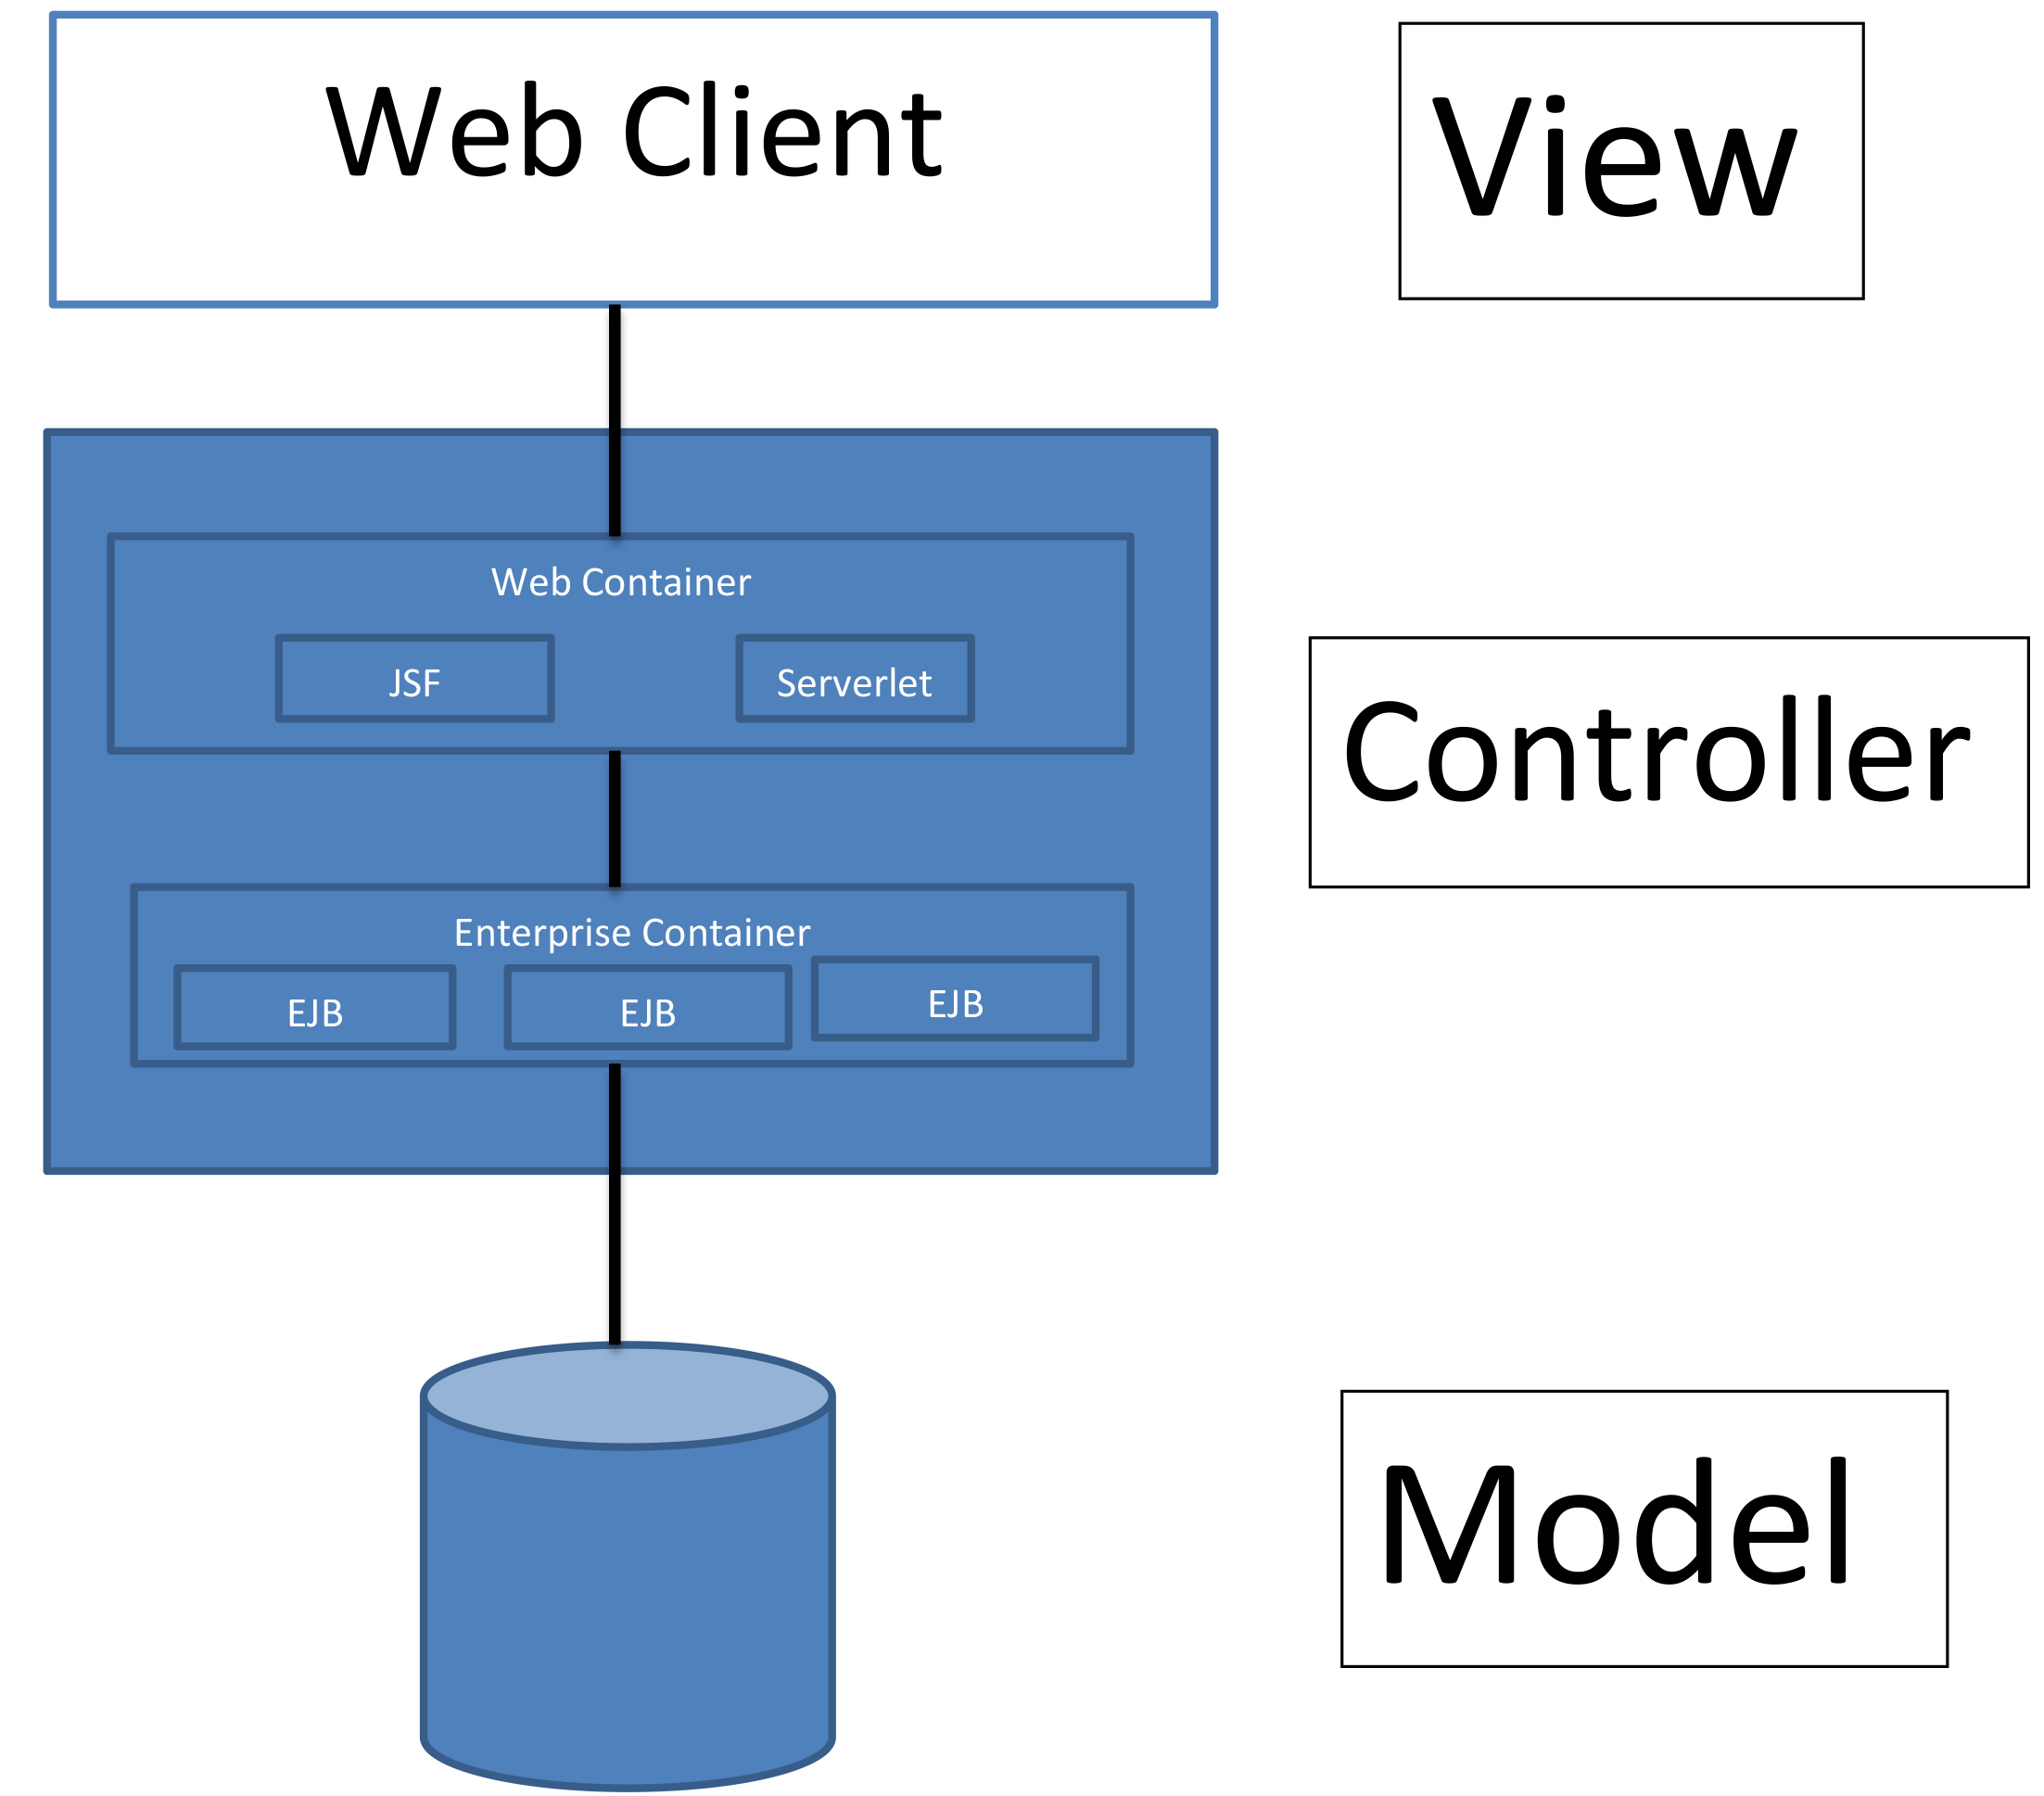
\includegraphics[scale=0.2]{../Images_Docs/Diagrams/Architecture/MVC.jpg}
\caption{Model View Controller of Architecture}
\end{figure}

\subsection*{View}
This component provides an interface to the under laying system to the user. This client is the web browser. It also incorporates components which are in the Web container(controller), such as Java Sever Faces. 
\subsection*{Controller}
This component is made up of two containers, the web container and the Enterprise container.
% More bullshit goes here.
\subsection*{Model}
This component is the actual database on which the system runs on. Which will be used as the centralised point of access with regards to applications being processed by the system as required by \client .
 
%%%%%%%%%%%%%%%%%%%%%%%%%%%%%%%%%%%%%%%%%%%%%%%%%%%%%%%%%%%%%%%%%%%%%%%%%%%%%%%%%%%%%%%%%%%%%%%%%%%%%%%%%%%%%
\section{Architectural Tactics and Strategies} % skipped till further notice.
This section describes techniques which will be used to satisfy the quality requirements. 

% This section needs a lot of paraphrasing...
\subsection{Concurrency}
The Java Platform has always offered support for concurrent programming, which is the basis for implementing many of the services offered by Java EE containers. This is realized through the two main concepts of having a multiple threads execute under a single process, in the case of Java EE mulitple beans execute under the JVM. The number of threads that can execute under the JVM can go well beyond thousands depending on factors such as the machine the JVM is running on and how it has been configured.\\

Even though the concurrent threads will mean better performance and a scalable implementation for the system they may lead to issues that effect the reliability and integrity of the system such as:
\begin{itemize}
\item Deadlocks,
\item Thread Starvation,
\item Concurrent  accessing of shared resources, and
\item Situations where the program generates incorrect data.
\end{itemize}

To deal with these issues Java EE provides concurrent utilities that access concurrent resources via JNDI lookup or resource injection. The components in the utilities ensure that the issues mentioned above are nullified. The primary components of interest in the concurrent utilities for our system are:
\begin{itemize}
\item managed executor service, 
\item managed scheduled executor service, 
\item managed thread factory, and 
\item context service.
\end{itemize}

\subsubsection{Managed Executor Service}
A managed executor service is used by applications to execute submitted tasks asynchronously. Tasks are executed on threads that are
started and managed by the container. The context of the container is propagated to the thread executing the task.

For example, by using an ManagedExecutorService.submit() call, a task, such as the GenerateReportTask, could be submitted to execute at a later time and then, by using the Future object callback, retrieve the result when it becomes available ().

\subsubsection{Managed Scheduled Executor Service}
A managed scheduled executor service is used by applications to execute submitted tasks asynchronously at specific times. Tasks are executed on threads that are started and managed by the container. The context of the container is propagated to the thread executing the task. The API
provides the scheduling functionality that allows users to set a specific date/time for the Task execution programmatically in the application.

\subsubsection{Managed Thread Factory}
A managed thread factory is used by applications to create managed threads. The threads are started and managed by the container. The context of the container is propagated to the thread executing the task. This object can also be used to provide custom factories for specific use cases (with custom Threads) and, for example, set specific/proprietary properties to these objects (Cervera-Navarro, Evans, Jendrock, Haase and Markito 2014).


%%%%%%%%%%%%%%%%%%%%%%%%%%%%%%%%%%%%%%%%%%%%%%%%%%%%%%%%%%%%%%%%%%%%%%%%%%%%%%%%%%%%%%%%%%%%%%%%%%%%%%%%%%%%%
\section{Use of Reference Architecture and Framework}
Java EE provides an API and runtime environment for developing and running large-scale, multi-tiered, scalable, reliable, and secure network applications. It also provides an architecture for implementing services as multitier applications that deliver the scalability, accessibility, and manageability needed by the system. This is reason to why it is ideal to use it in the development of the project.

It allows easy development of thin-client multi tiried applications without the many lines of complicated code that handles transactions or state management. Business logic is organized into reuseable components and provides underlying services as containers for all component types.

The features in the JavaServer Faces technology provided HTML5 friendly markup which will assist in the implementation of the user friendly UI.

\subsection{Java Persistence}
Java EE is in itself implemented as a object oriented model, yet it is expected to function with mainly relational databases. To bridge the gap between an object-oriented model and a relational database an object/relational mapping approach will be used to achieve Persistence. Java Persistence consists of the following areas:
\begin{itemize}
\item The Java Persistence API,
\item The query language, and
\item Object/relational mapping metadata
\end{itemize}

\subsection{RESTful web services}
RESTful web services are loosely coupled, lightweight web services that are particularly well suited for creating APIs for clients spread out across the internet. Representational State Transfer (REST) is an architectural style of client-server application centered around the transfer of representations of resources through requests and responses. In the REST architectural style, data and functionality are considered resources and are accessed using Uniform Resource Identifiers (URIs), typically links on the Web. The resources are represented by documents and are acted upon by using a set of simple, well-defined operations.

In Java EE 7, JAX-RS provides the functionality for Representational State Transfer (RESTful) web services. JAX-RS is a Java programming language API designed to make it easy to develop applications that use the REST architecture.

The JAX-RS API uses Java programming language annotations to simplify the development of RESTful web services. Developers decorate Java programming language class files with JAX-RS annotations to define resources and the actions that can be performed on those resources. JAX-RS annotations are runtime annotations; therefore, runtime reflection will generate the helper classes and artifacts for the resource. A Java EE application archive containing JAX-RS resource classes will have the resources configured, the helper classes and artifacts generated, and the resource exposed to clients by deploying the archive to a Java EE server (Cervera-Navarro, Evans, Jendrock, Haase and Markito 2014).

%%%%%%%%%%%%%%%%%%%%%%%%%%%%%%%%%%%%%%%%%%%%%%%%%%%%%%%%%%%%%%%%%%%%%%%%%%%%%%%%%%%%%%%%%%%%%%%%%%%%%%%%%%%%%
\section{Access and Integration channels}
This section discusses the requirements for the channels through which the system can be accessed by humans and other systems. Also making mention about the integration channels which need to be followed. 

\subsection{Access Channels}
The system will be accessible by humans through the recent versions of the following browsers:
\begin{enumerate}
\item Mozilla Firefox,
\item Google Chrome,
\item Microsoft Internet Explorer
\item Apple Safari, and
\item Opera
\end{enumerate}
The mobile counterparts of the above mentioned browsers will also be catered for and so no other access channel (such as Android/Apple apps) is to be considered.
\subsection{Integration Channels}
Upon successful complementation the system must be integratedable with the University of Pretoria's PeopleSoft system. Therefore it is sensible to implement the system in Java EE as it is one of the many components that form part of the multiple tiers that build up  PeopleSoft. \\
\\
The use of build tools such as Maven will provide a central piece of information with regards to the projects build, reporting and documentation. This central point of information will assist in the integration phase since it is implemented through a standardised build approach which can come into play at a later time through the use of EAI.\\
\\
The EAI will be achieved via  the logical integration architecture of Direct point-to-point integration (Kang, 2002). This means that the application management system will make direct JDBC calls to the universities databases tables (which needed to be setup to cater for our system at that point). The Integration method will be pushed-based data-level integration (or if all else fails UI-Level integration).
% http://www.javaworld.com/article/2074488/enterprise-java/enterprise-application-integration-using-j2ee.html

\section{Technologies}
The System will use the following technologies:
\begin{itemize}
\item Java Enterprise Edition 7, 
\item MySQL database, open-source relational database management system
\item Netbeans 8.0
\item Glassfish server
\end{itemize}

\subsection*{Integrated Development Environment}
The system should be buildable independent of an IDE but it will be developed on Netbeans 8.0 to allow for uniformity amongst the development team, with regards to coding style, and provide easy integration with the tools that will be used such as Javadoc, to generate  API documentation in HTML format.

\subsection*{API}
\begin{itemize}
\item Java Persistence API. The Java Persistence API (JPA) is a Java standards–based solution for persistence.
\item JavaMail. API used to send email notifications.
\item JavaBeans Activation Framework. The JavaBeans Activation Framework (JAF) is used by the JavaMail API. JAF provides standard services to determine the type of an arbitrary piece of data, encapsulate access to it, discover the operations available on it, and create the appropriate JavaBeans component to perform those operations.
\item Java Database Connectivity. The Java Database Connectivity (JDBC) API lets you invoke SQL commands from Java programming language methods. You use the JDBC API in an enterprise bean when you have a session bean access the database. You can also use the JDBC API from a servlet or a JSP page to access the database directly without going through an enterprise bean.
\item Java Naming and Directory Interface. The Java Naming and Directory Interface (JNDI) API provides naming and directory functionality, enabling applications to access multiple naming and directory services, such as LDAP, DNS, and NIS. The JNDI API provides applications with methods for performing standard directory operations, such as associating attributes with objects and searching for objects using their attributes. Using JNDI, a Java EE application can store and retrieve any type of named Java object, allowing Java EE applications to coexist with many legacy applications and systems.
\item Java API for XML Web Services. The Java API for XML Web Services (JAX-WS) specification provides support for web services that use the JAXB API for binding XML data to Java objects. The JAX-WS specification defines client APIs for accessing web services as well as techniques for implementing web service endpoints. The Implementing Enterprise Web Services specification describes the deployment of JAX-WS-based services and clients. The EJB and Java Servlet specifications also describe aspects of such deployment. JAX-WS-based applications can be deployed using any of these deployment models.
\item SOAP with Attachments API for Java. The SOAP with Attachments API for Java (SAAJ) is a low-level API on which JAX-WS depends. SAAJ enables the production and consumption of messages that conform to the SOAP 1.1 and 1.2 specifications and the SOAP with Attachments note.
\item Java Authentication and Authorization Service. The Java Authentication and Authorization Service (JAAS) provides a way for a Java EE application to authenticate and authorize a specific user or group of users to run it.
\end{itemize}

\subsection*{Build Tools}
\begin{itemize}
\item Apache Maven (for reasons explained in the integration channels section).
\end{itemize}

\subsection*{Operating System}
The system will be deployable on:
\begin{itemize}
\item Windows 7 and 8.
\item Linux based operating systems (specifically Kububuntu 13).
\end{itemize}
\newpage

\section{Glossary:} %Mathys
\vspace{0.2in}

\begin{itemize}

\item \textbf{API} - Application Programming Interface
\item \textbf{Application} -Both renewal applications or new fellowship applications are seen as applications by this project.
\item \textbf{CV} - Curriculum Vita
\item \textbf{EAI} - Enterprise Application Integration
\item \textbf{HTML} - Hyper Text Mark-up Language
\item \textbf{Java EE} - Java Enterprise Edition
\item \textbf{JDBC} - Java Database Connection
\item \textbf{MVC} - Model View Controller
\item \textbf{UI} - User Interface
\item \textbf{UP} - University of Pretoria
 
\end{itemize}	

\end{document}